\documentclass[en]{../../../../../../eplexam}

\hypertitle{analog}{8}{ELEC}{2532}{2021}{Juin}{All}
{Maxime Leurquin}
{Denis Flandre, David Bol}

\section{Crise covid modalités}
L'examen s'est fait en présentiel et durait 3h. Calculatrice autorisée.

\part{Theory}

\section{Question 1}


\begin{figure}[h]
    \centering
    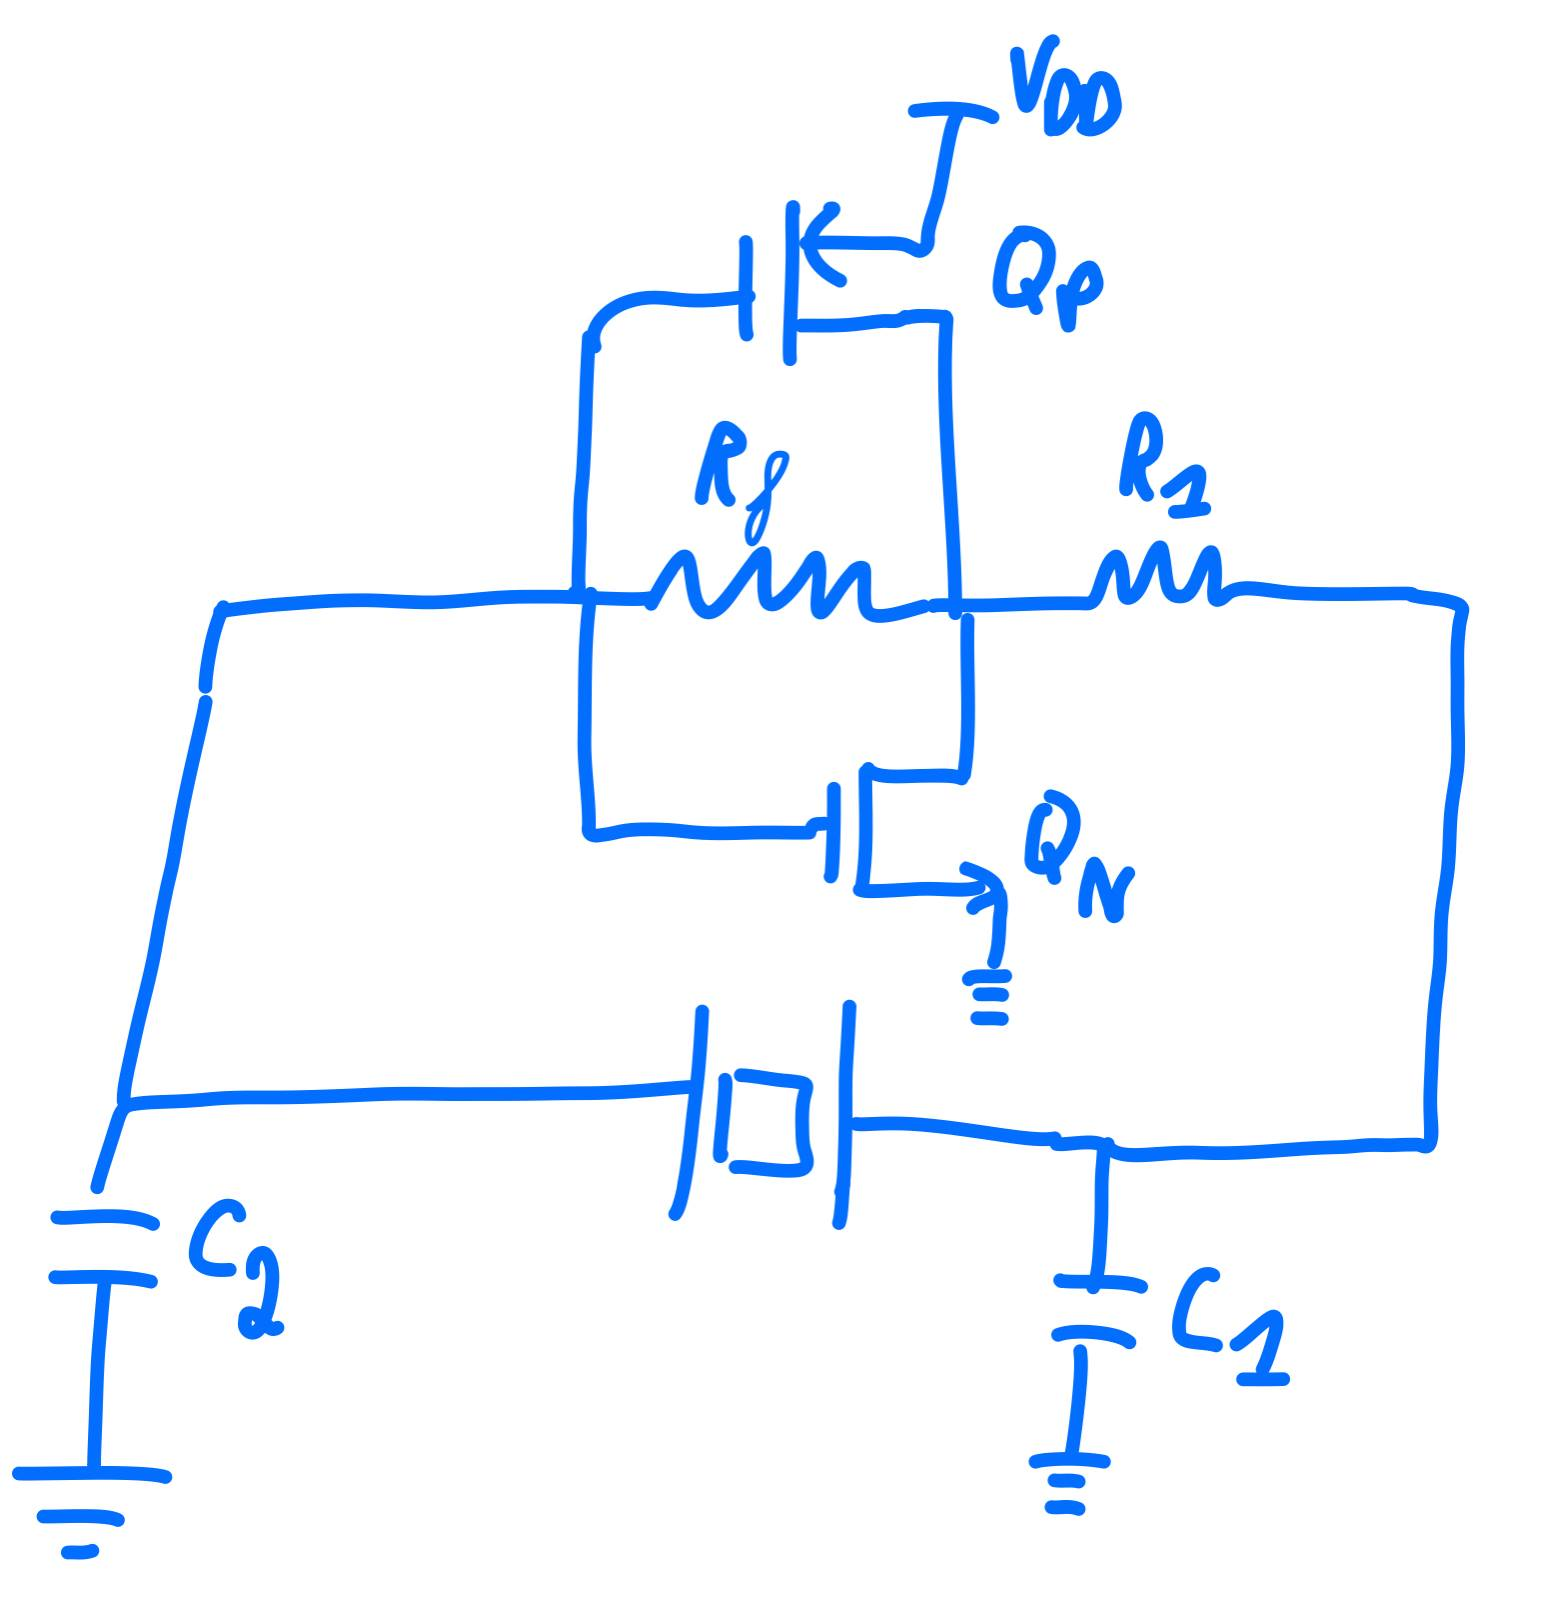
\includegraphics[width=0.5\textwidth]{TheoryQ1.jpg}
    \caption{Circuit theory question 1}
\end{figure}

\begin{enumerate}
\item Using a conceptual diagram, explain the function, the different blocks, the operation and application of the circuit below.
\item Give and explain the most important criterion and equation used to determine the values of the circuit components in order to achieve its main first order specifications.
\end{enumerate}

% Insérer ci-dessous la solution à la question
%\begin{solution}
%mysolution....
%\end{solution}

\nosolution



\section{Question 2}

\begin{enumerate}
\item Draw the schematic of a simple, though complete current source or reference.
\item Briefly discuss its behavior and performance using graphs and equations.
\item Give some typical numerical values.
\end{enumerate}

% Insérer ci-dessous la solution à la question
%\begin{solution}
%mysolution....
%\end{solution}

\nosolution

\part{Practice}
\section{Question 1 [/5]}
\noindent The butterworth filter is a type of linear analog filter designed to have a frequency response as flat as possible in the pass band. As a reminder the transfer function $H(j\omega)$ of a low pass filter of order $n$ is : $$H(j\omega)=\frac{1}{\sum^n_{i=0}a_i\left(\frac{j\omega}{\omega_c}\right)^i}$$
where $\omega_c$ is the cutoff and $a_i$ are chosen to reach the wanted performances. For a butterworth filter the coefficients are given in table \ref{butt}.

\noindent The sallen and key is an electronic filter topology that can be used to implement any linear second order analog filter. This circuit is made with an operational amplifier and 4 passive components. The low pass circuit is given below.
\begin{figure}[h]
    \centering
    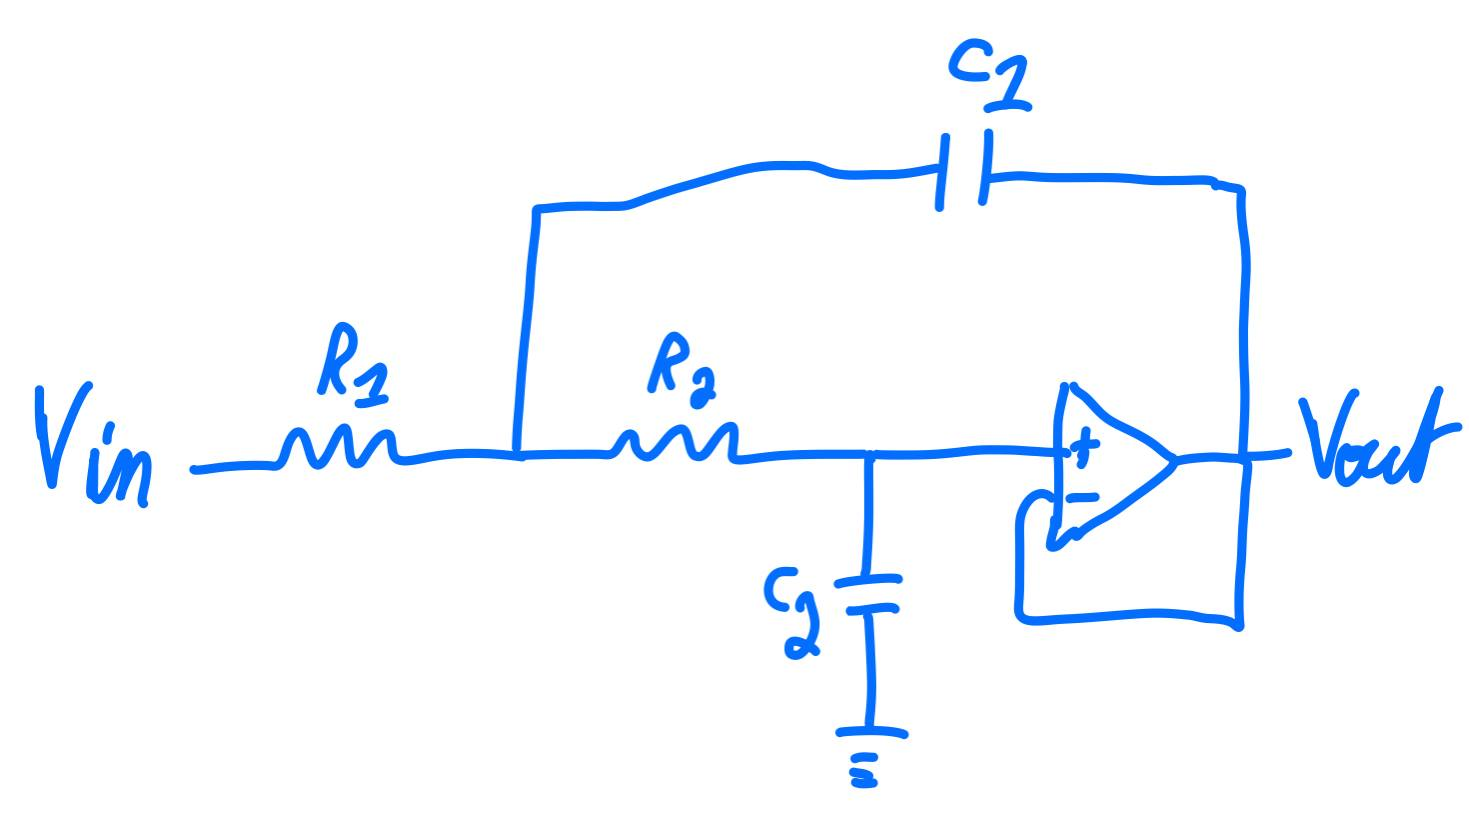
\includegraphics[width=0.5\textwidth]{SallenKey.jpg}
    \caption{Sallen and Key circuit.}
\end{figure}

\noindent For this question you will be asked to implement a second order low pass butterworth filter with a cutoff of 10kHz using the Sallen and Key topology.\\


\begin{table}[!ht]
\begin{tabular}{c|cccccc}
n & $a_0$ & $a_1$      & $a_2$ & $a_3$ & $a_4$ & $a_5$ \\ \hline
1 & 1     & 1          &       &       &       &       \\
2 & 1     & $\sqrt{2}$ & 1     &       &       &       \\
3 & 1     & 2          & 2     & 1     &       &       \\
4 & 1     & 2.613      & 3.414 & 2.613 & 1     &       \\
5 & 1     & 3.236      & 5.236 & 5.236 & 3.236 & 1    
\end{tabular}
\centering
\caption{Butterworth filter coefficients}
\label{butt}
\end{table}


\begin{enumerate}
\item Write the general transfer function of a second order low pass filter in terms of $\omega_c$, $\omega$ and damping factor $\xi$ [/0.5]

\item  Give the expression of the poles in terms of $\xi$ and $\omega_c$. Discuss the stability and time response of the filter depending on the value of $\xi$ and give the value of $\xi$ for a butterworth filter.\footnote{if you don't remember the expression with $\xi$ do it in terms of $a_0,a_1,a_2$}[/1.5]


\item Find $H(j\omega)=\frac{v_{out}(j\omega)}{V_{in}(j\omega)}$ of the Sallen-key filter [/1.5]

\item Find the value of $R_1$ and $C_1$ if you have $R_2=1k\Omega$,$C_2=1nF$ in order to have a second order butterworth filter with a cutoff frequency of 10kHz [/1.5]

\end{enumerate}



% Insérer ci-dessous la solution à la question
%\begin{solution}
%mysolution....
%\end{solution}

\nosolution



\section{Question 2 [/5]}

\begin{figure}[h]
    \centering
    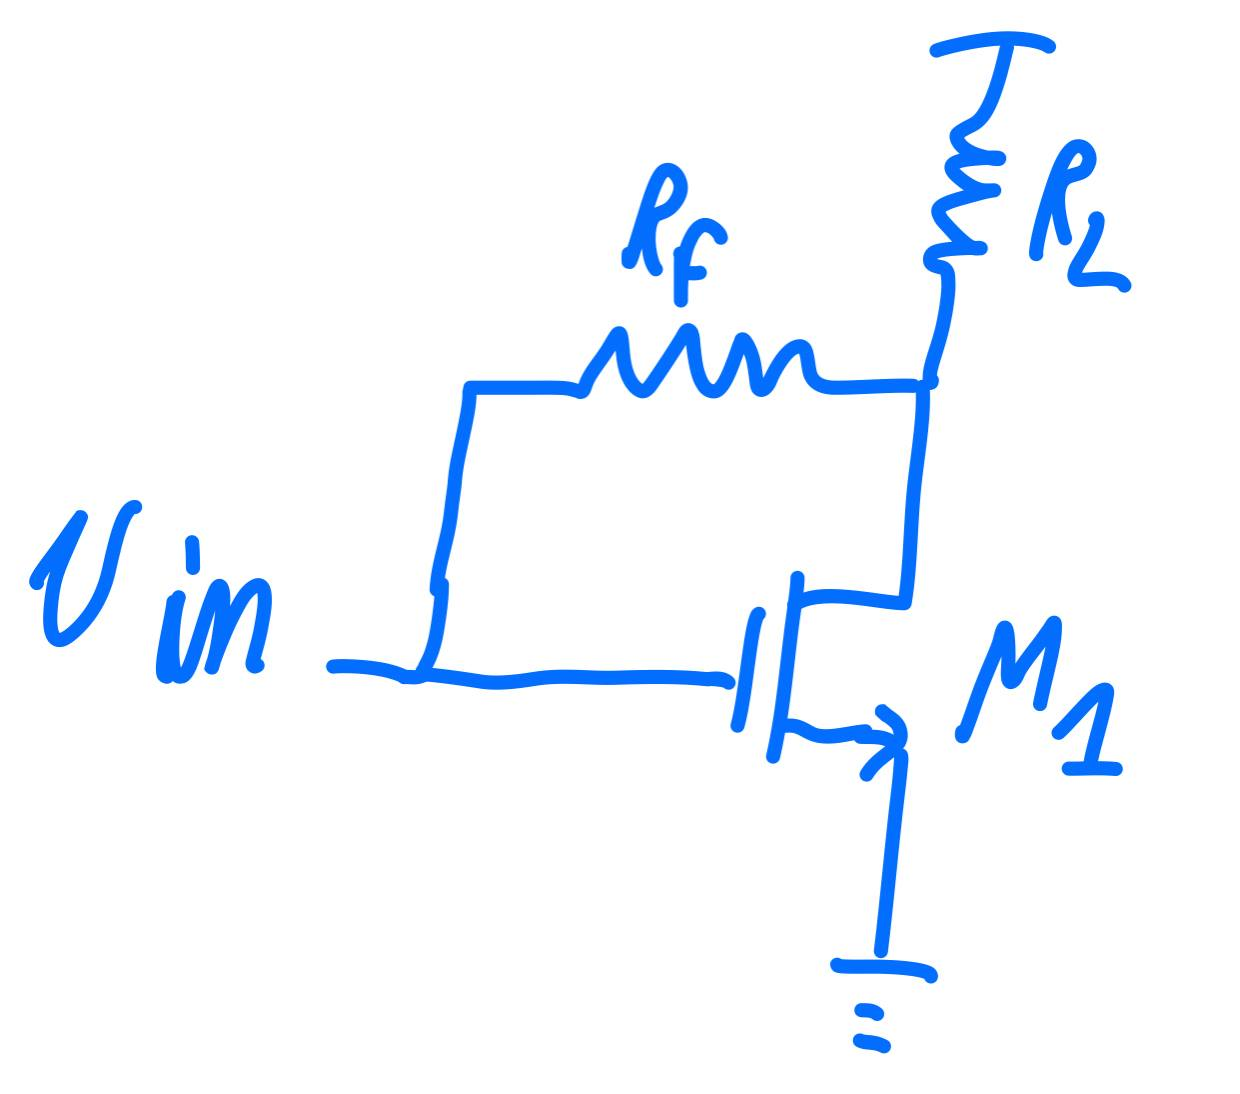
\includegraphics[width=0.5\textwidth]{ExNoise.jpg}
    \caption{Shunt feedback amplifier}
\end{figure}

Here is a shunt-feedback amplifier, a basic topology for a Low Noise Amplifier (LNA). The transfer function without considering the noise sources is given by $\frac{V_{out}}{V_{in}}=\frac{1-g_mR_F+j\omega R_FC_{gd}}{1+\frac{R_F}{R_L}j\omega R_FC_{gd}}$. Early and the leakage current are neglected.



\begin{enumerate}
\item Identify all the noise sources of the circuit and give the expression and units of their power spectral density [/1]
\item Sketch the power spectral density of the noise of the transistors. Identify in this plot the main characteristics of the PSD [/1]
\item Obtain the expression of the power spectral density of the equivalent input refered noise voltage source $v_n$ of the circuit. Explain clearly the procedure followed. Do not forget any noise source. [/3]
\end{enumerate}


% Insérer ci-dessous la solution à la question
%\begin{solution}
%mysolution....
%\end{solution}

\nosolution


\end{document}
